The final step in the bending process is the controlled placement of the bent parts in the storage station. The storage station is a shelf with ten drawers. The robot gripper is used to open and close a drawer of the shelf.
Before the placement of the bent sheet metal part, an empty drawer is open. Figure \ref{fig:shelf-control} illustrates the steps taken by the robotic gripper to open an empty drawer of the shelf. Once the drawer is open, it doesn't move because of a locking mechanism. After a drawer is completely filled, robotic gripper is used again to close the drawer. The steps are similar to opening of shelf but in reverse order.
\FloatBarrier
\begin{figure}[!ht]
    \centering
    \begin{subfigure}[b]{0.32\textwidth}
        \centering
        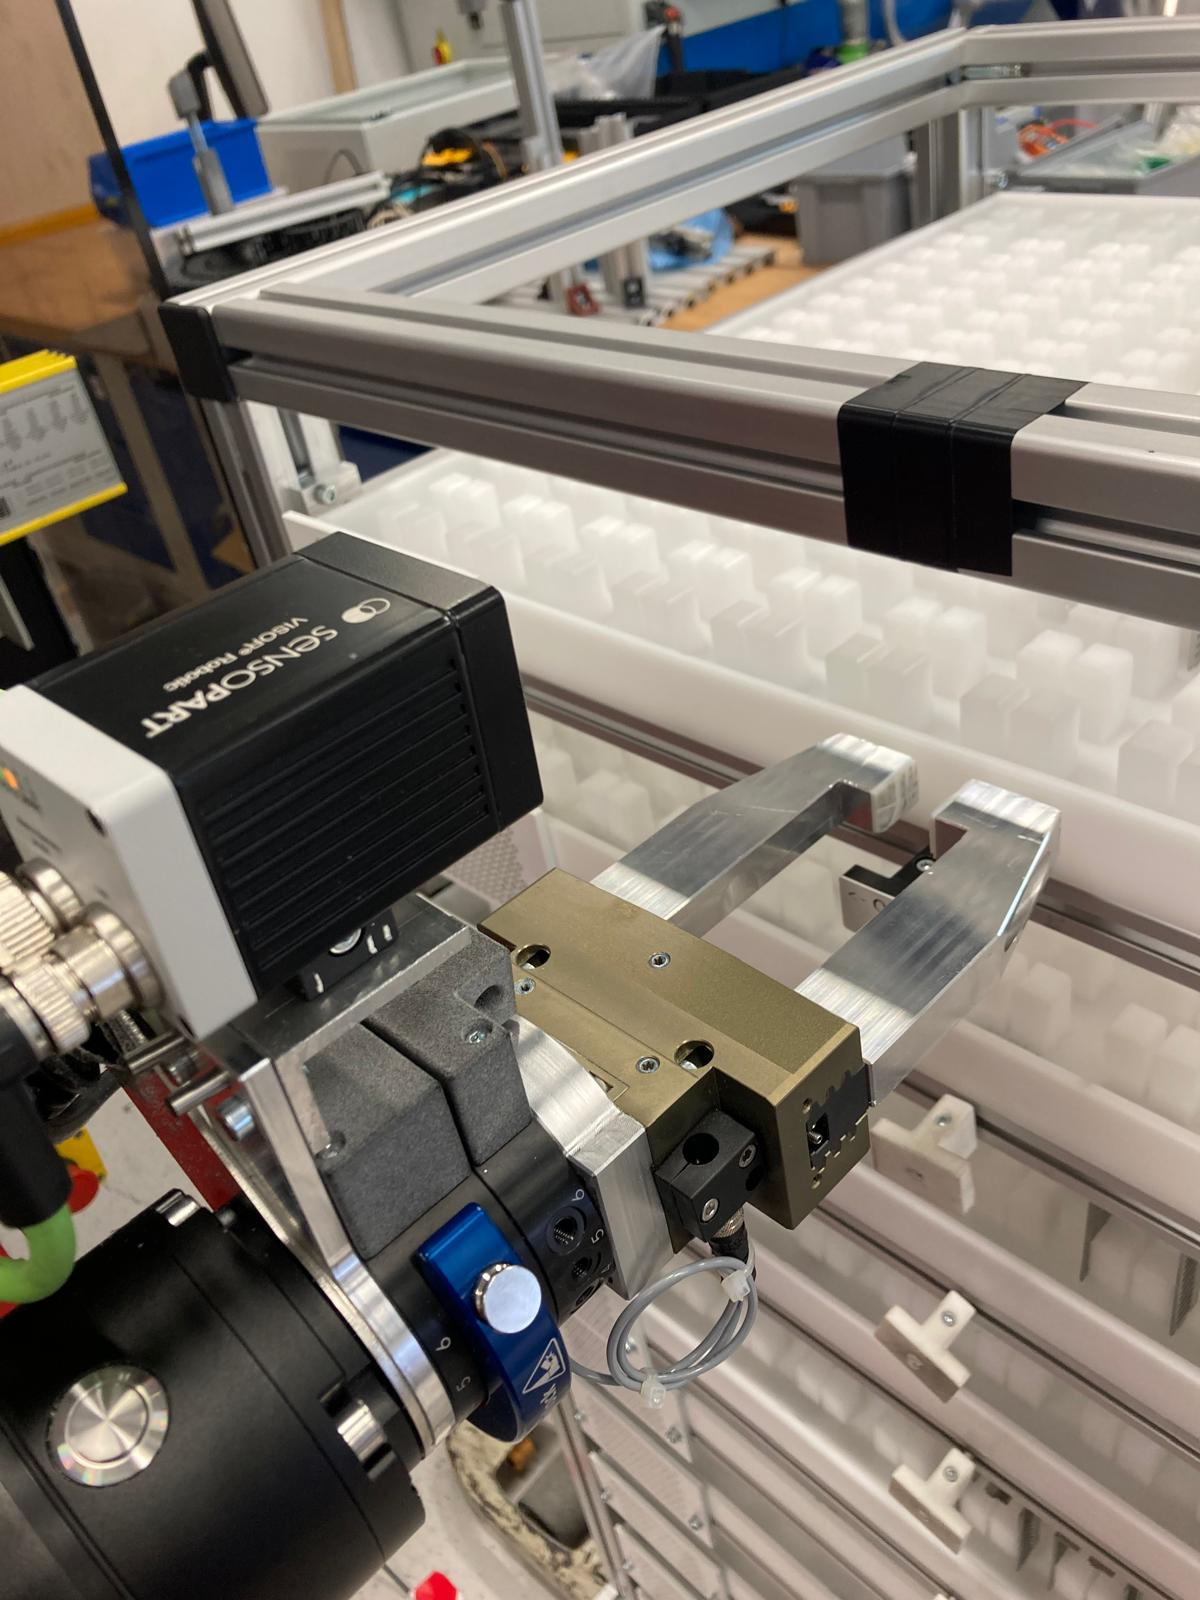
\includegraphics[width=\textwidth]{figures/shelf-control/reach-handle.jpeg}
        \caption{Reach shelf handle}
        \label{subfig:reach-handle}
    \end{subfigure}\hspace{0.1cm}
    \begin{subfigure}[b]{0.32\textwidth}
        \centering
        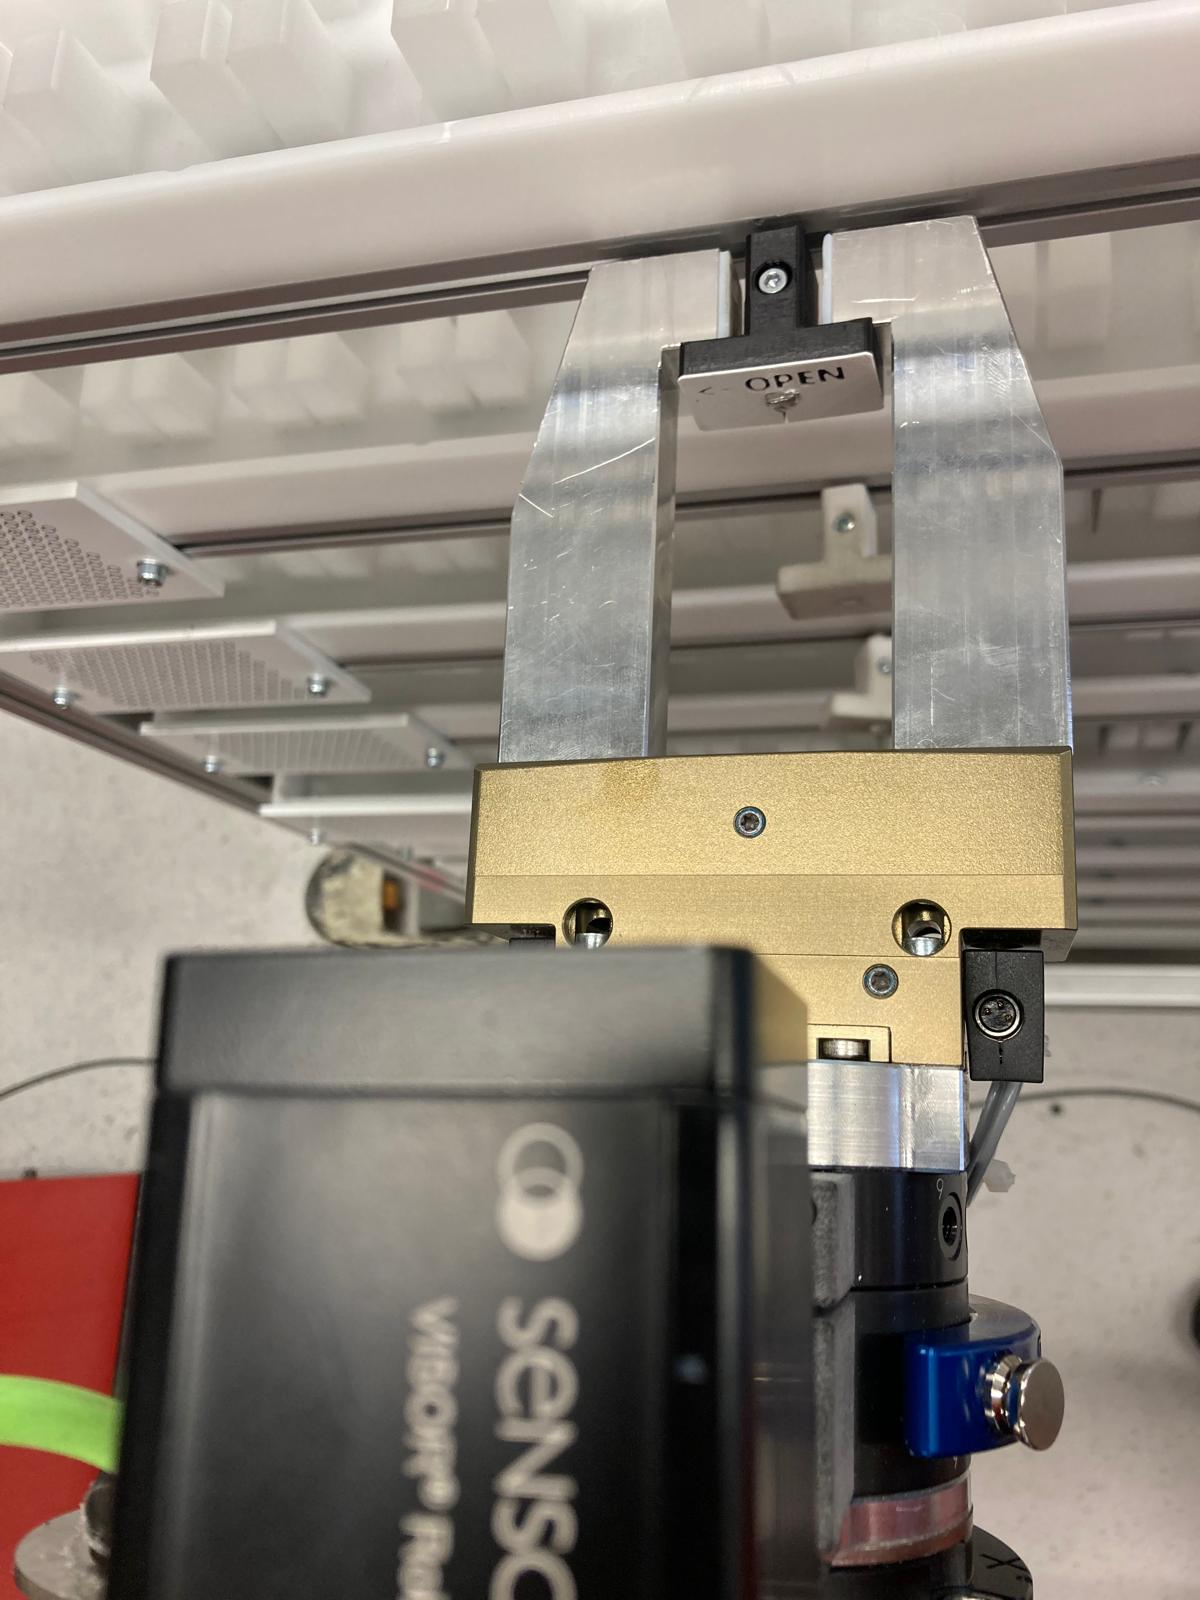
\includegraphics[width=\textwidth]{figures/shelf-control/hold-handle.jpeg}
        \caption{grasp handle with gripper}
        \label{subfig:grasp-handle}
    \end{subfigure}\hspace{0.1cm}
    \vspace{1cm}
    \begin{subfigure}[b]{0.32\textwidth}
        \centering
        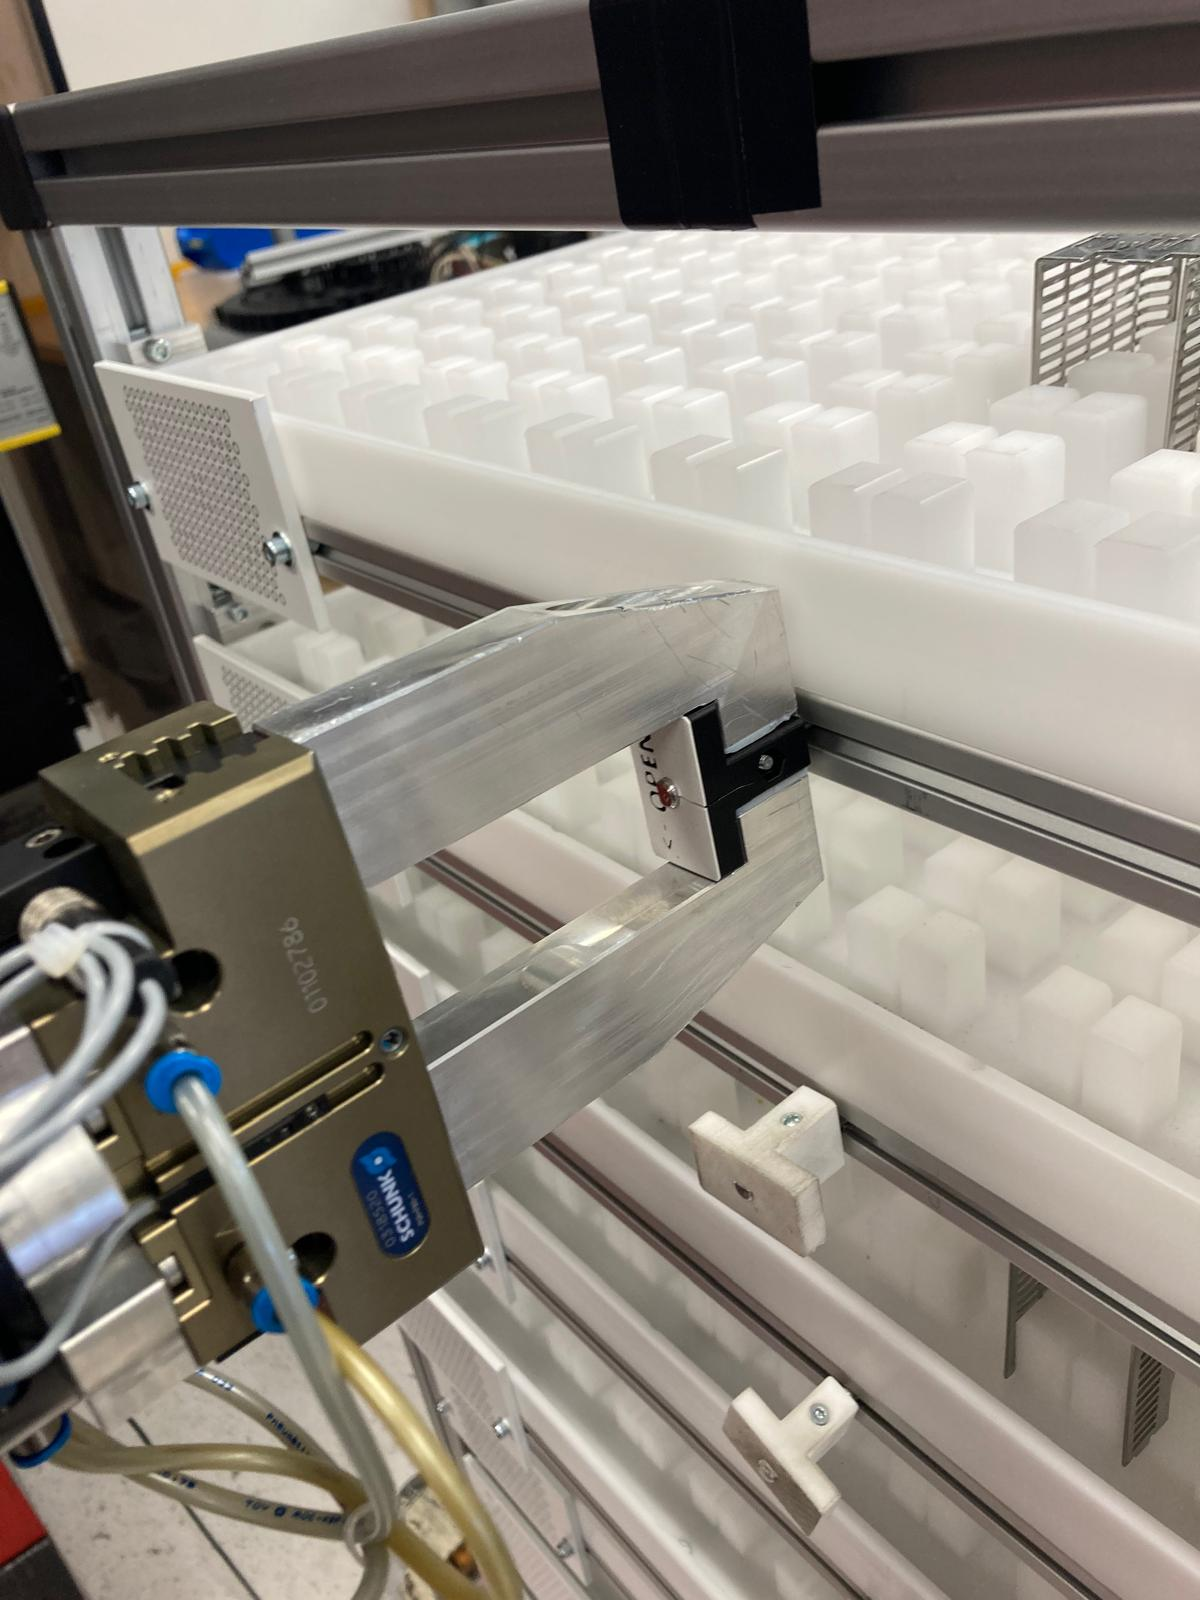
\includegraphics[width=\textwidth]{figures/shelf-control/open-handle.jpeg}
        \caption{Turn handle 100\textdegree{} to open drawer}
        \vspace{-0.45cm}
        \label{subfig:turn-open}
    \end{subfigure}\hspace{0.1cm}
    \begin{subfigure}[b]{0.32\textwidth}
        \centering
        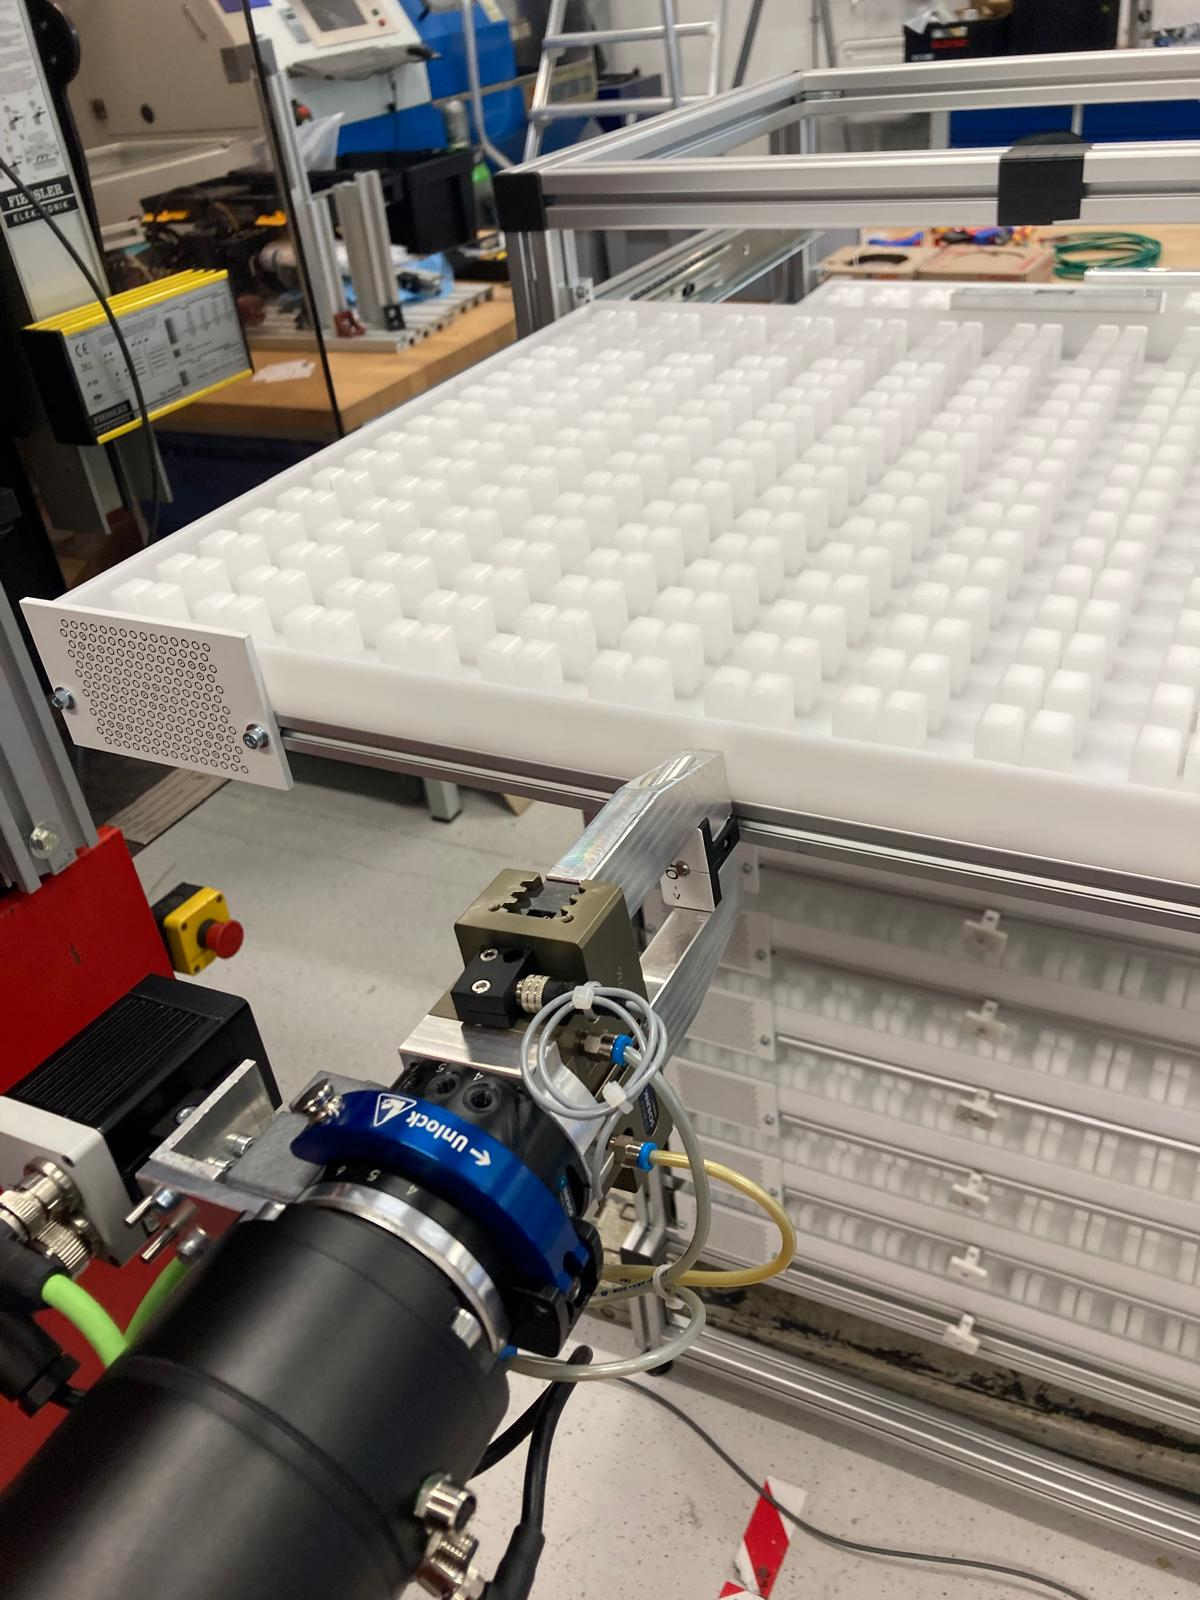
\includegraphics[width=\textwidth]{figures/shelf-control/open-drawer.jpeg}
        \caption{open drawer}
        \vspace{0.45cm}
        \label{fig:open-drawer}
    \end{subfigure}\hspace{0.1cm}
    \vspace{0.75cm}
    \begin{subfigure}[b]{0.32\textwidth}
        \centering
        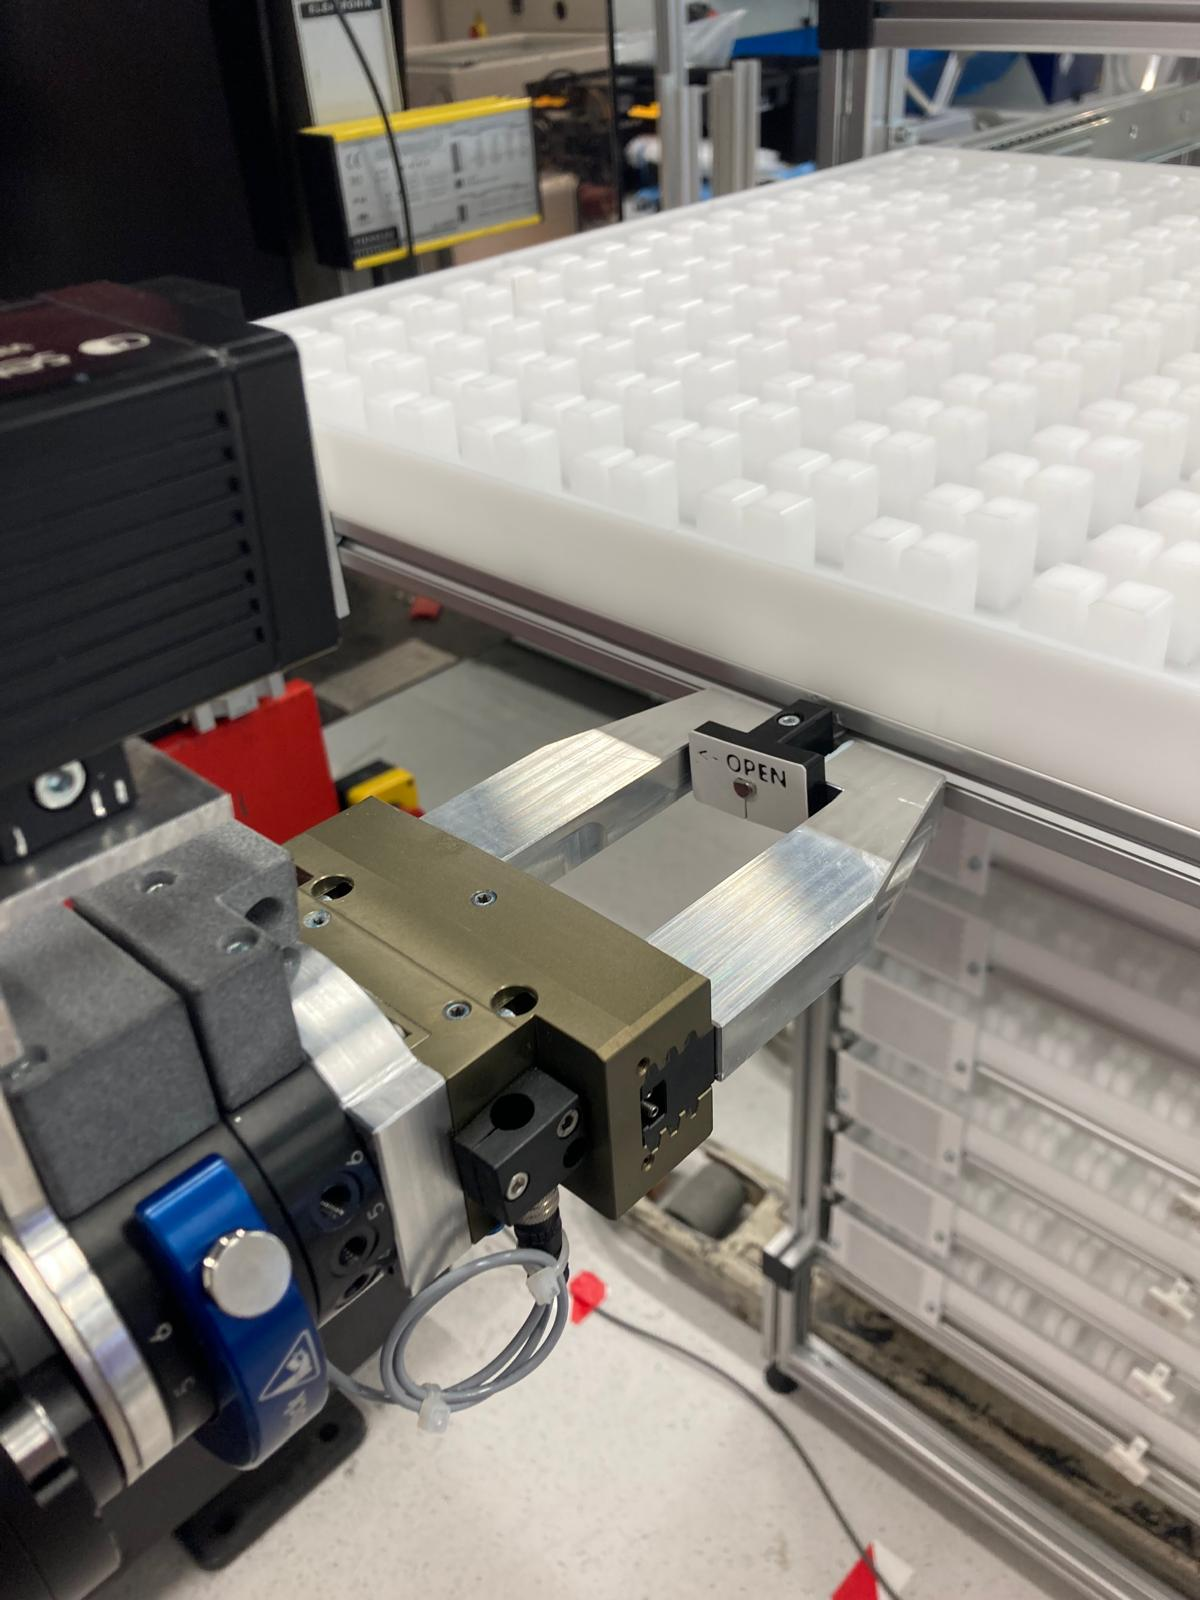
\includegraphics[width=\textwidth]{figures/shelf-control/close-handle.jpeg}
        \caption{Turn handle -100\textdegree{} to fix drawer in closed position}
        \label{fig:close-handle}
    \end{subfigure}\hspace{0.1cm}
    \begin{subfigure}[b]{0.32\textwidth}
        \centering
        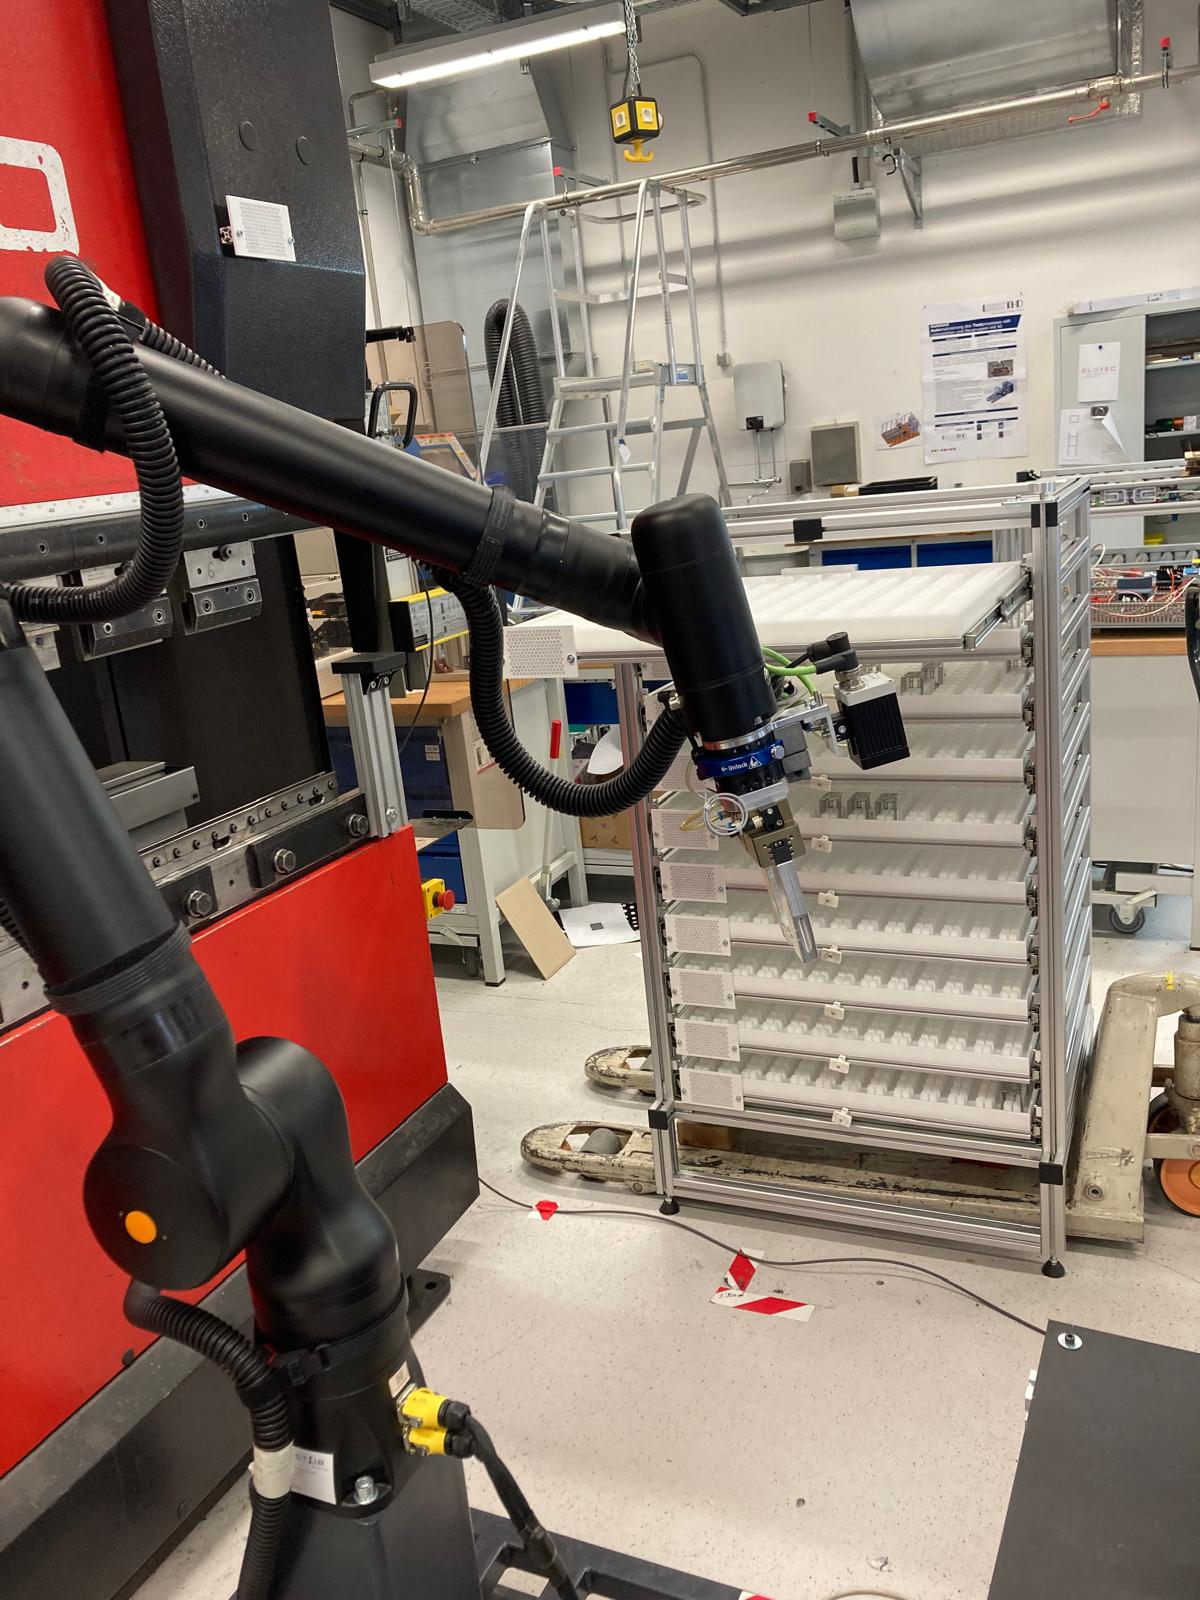
\includegraphics[width=\textwidth]{figures/shelf-control/drawer-opened.jpeg}
        \caption{Robot ready with drawer open}
        \label{subfig:drawer-opened}
    \end{subfigure}\hspace{0.1cm}
    \caption{Opening a shelf drawer for placement of bent sheet metal parts}
    \label{fig:shelf-control}
\end{figure}

\begin{figure}[!ht]
    \centering
    \begin{subfigure}[b]{0.48\textwidth}
        \centering
        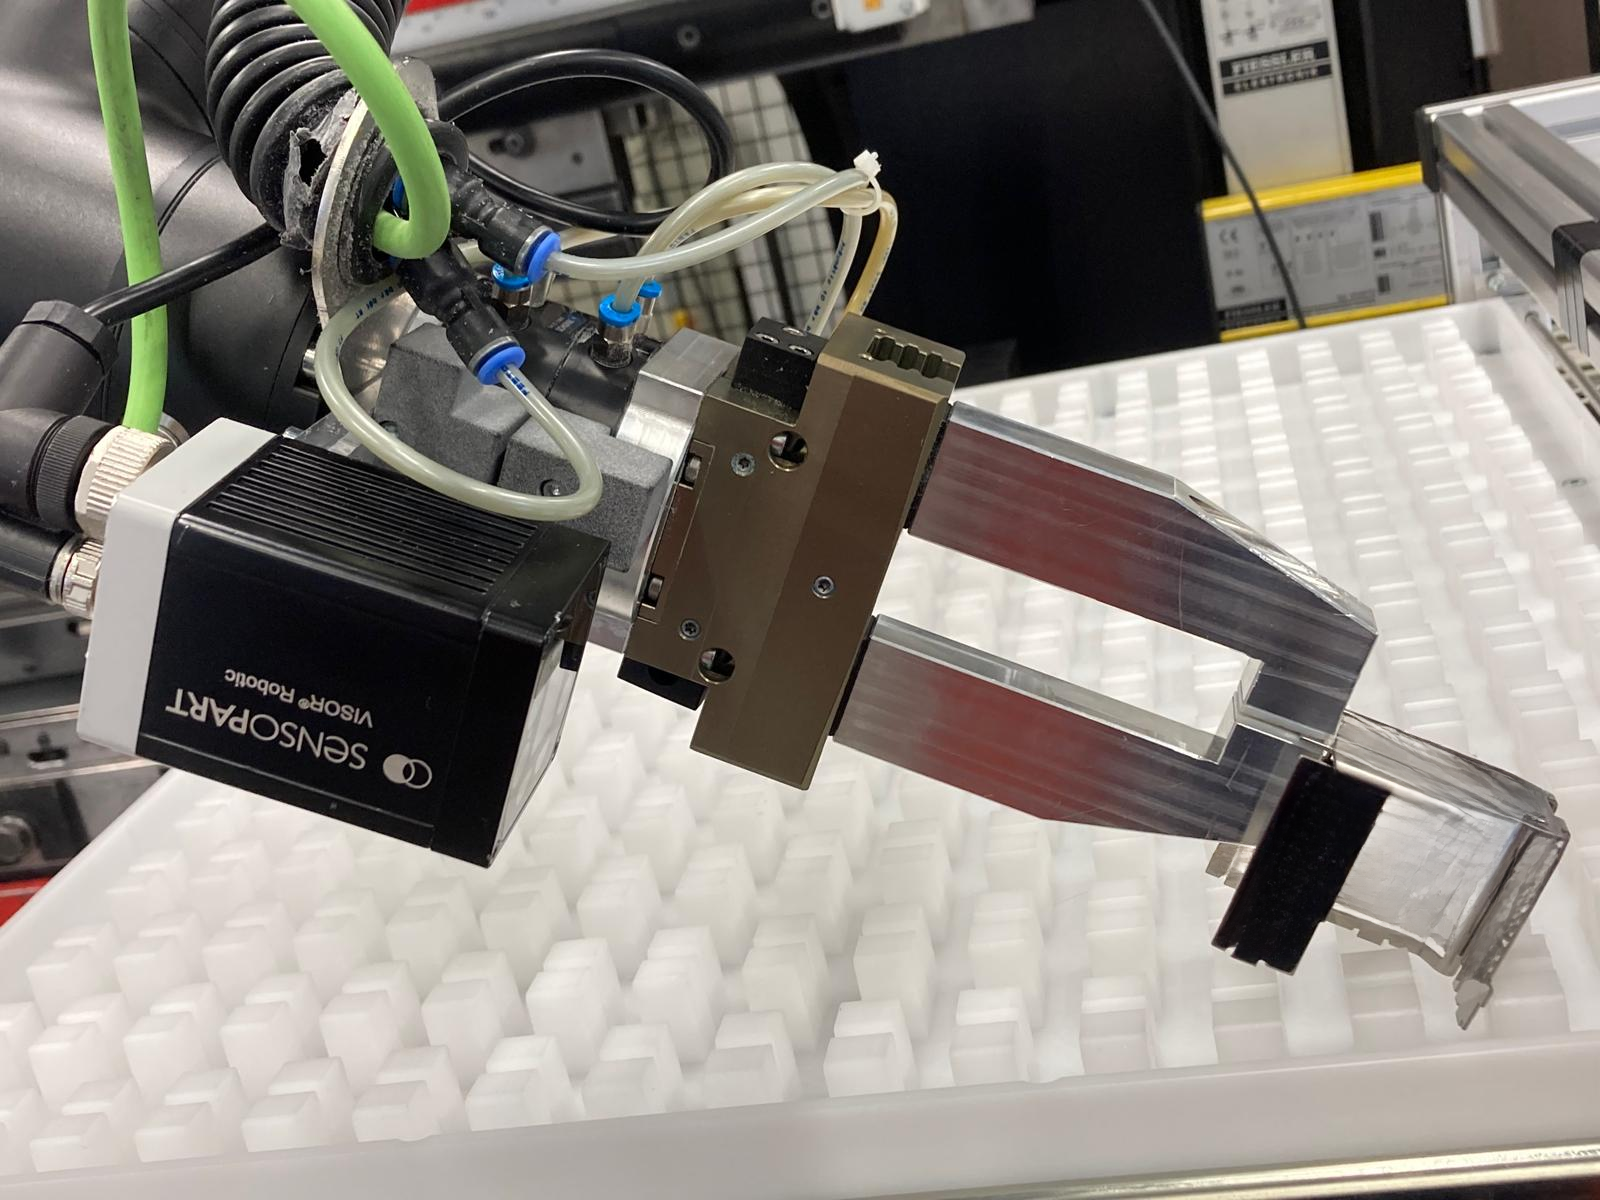
\includegraphics[width=\textwidth]{figures/shelf-control/sheet-placement-01.png}
        \caption{place bent sheet}
        \label{subfig:sheet-placement1}
    \end{subfigure}\hspace{0.1cm}
    \begin{subfigure}[b]{0.48\textwidth}
        \centering
        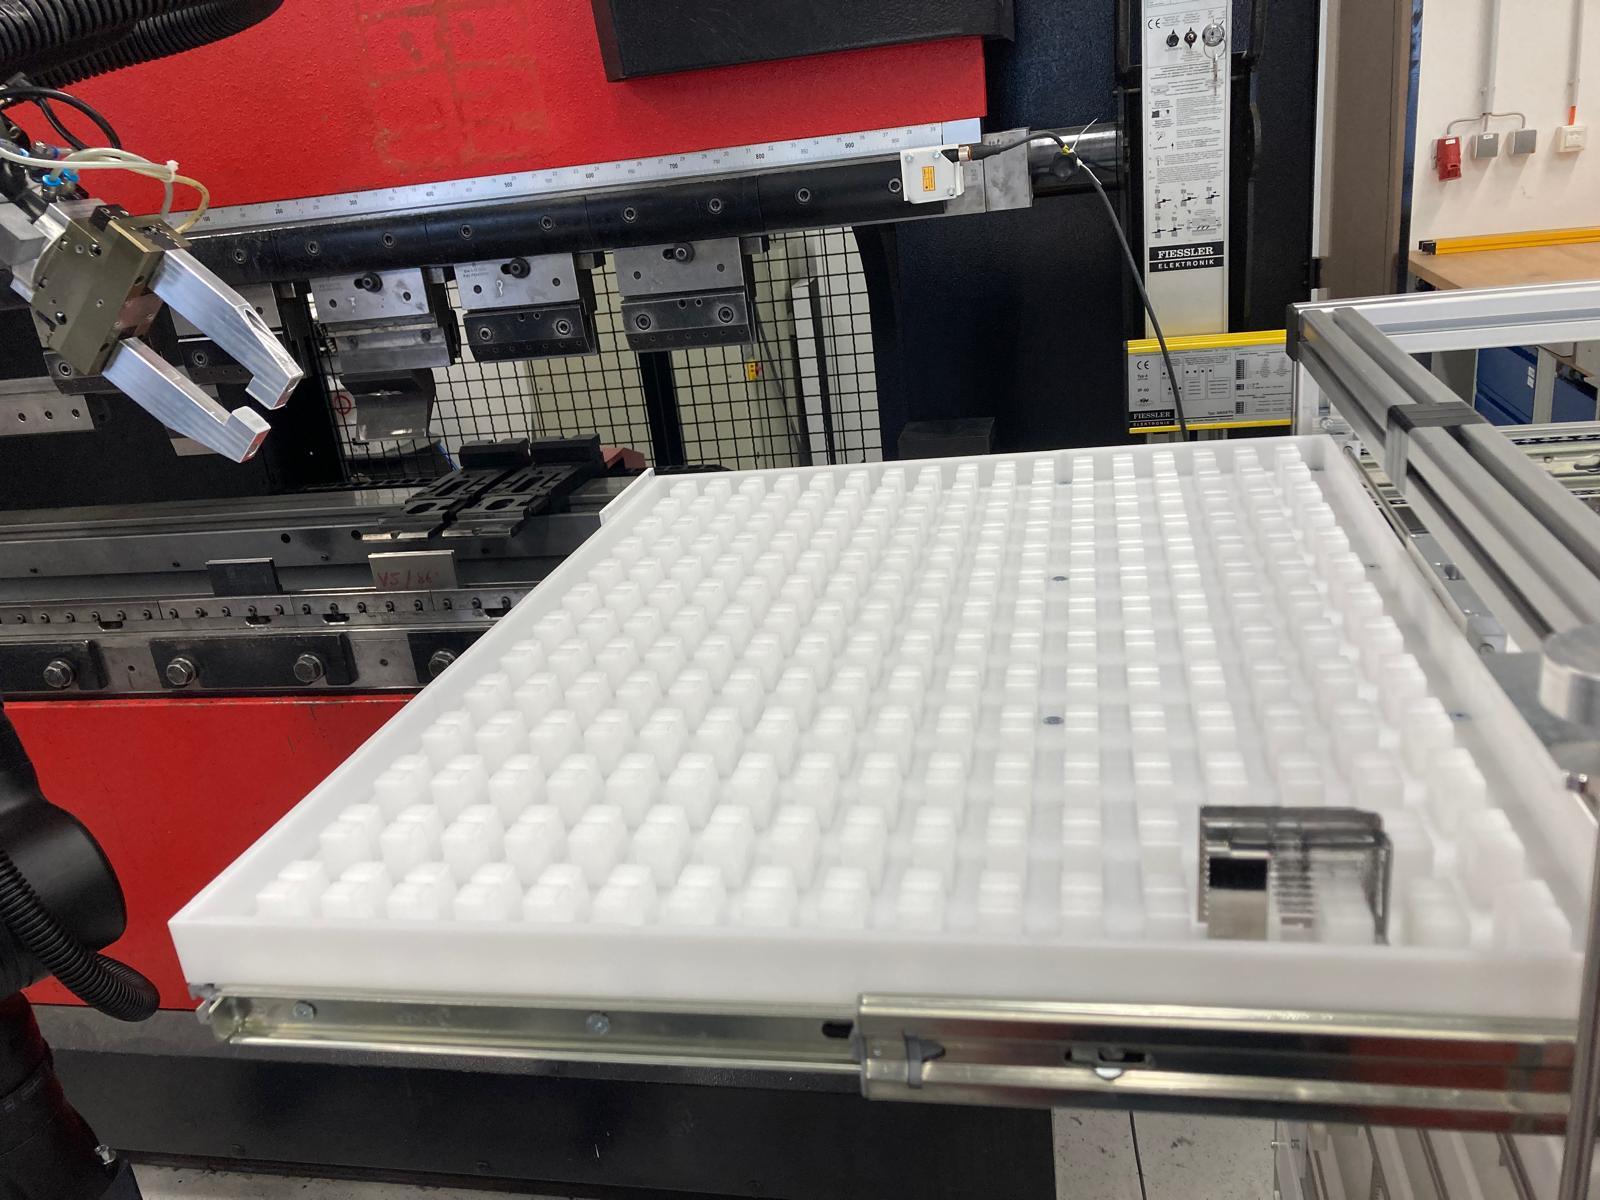
\includegraphics[width=\textwidth]{figures/shelf-control/sheet-placement-02.png}
        \caption{final position}
        \label{subfig:sheet-placement2}
    \end{subfigure}\hspace{0.1cm}
    \caption{Sheet placement}
    \label{fig:sheet-placement}
\end{figure}


Using a predefined pattern, the robot places each part onto the designated section on the drawer shelf, ensuring optimal space utilization. In total 65 parts can be placed in a single empty drawer, 13 in a single row and 5 in a column. So, in total the storage station with ten drawers has a capacity of 650 bent parts. The robot also keeps track of the number of parts produced and stored, with automatic handling of a drawer once a drawer is filled.

In the event that a shelf is full, the production is paused and the robot goes in a waiting state. It waits for the human operator to change the filled shelf with an empty one and update it on the SIMATIC HMI.

The placement of the test part marks the end of the bending cycle. After it is determined that all the bending operations and handling of shelf is working correctly, the production of a part can begin.
Th integration tests ensured that the entire workflow—from pickup, bending, inspection, to placement—is seamlessly integrated and automated.



